\chapter{Annex}

\begin{appendix}
	\section*{Appendix A}
	
	\caption{Pin configuration of PC104 connector}
	\begin{longtable}{p{3cm}p{6cm}}
		\toprule
		Pin & Description \\ \midrule
		C1-1 & PCU CAN1 Interface L \\ 
		C1-3 & PCU CAN1 Interface H \\ 
		C1-12 & JTDI\_OBC \\ 
		C1-13 & JTCK\_OBC \\ 
		C1-14 & JTMS\_OBC \\ 
		C1-15 & JTDO\_OBC \\ 
		C1-16 & JTRST\_OBC \\ 
		C1-17 & PCU UART1 Interface RX \\ 
		C1-18 & PCU UART1 Interface TX \\ 
		C1-27 & OBC Current Sensor \\ 
		C1-31 & PCU Watchdog Disable Pin \\ 
		C1-32 & EGSE Battery Charge Power Input \\ 
		C1-33 & Output Voltage HISPICO \\ 
		C1-34 & PCU CAN2 Interface L \\ 
		C1-35 & 3.3V PCU EPS JTAG \\ 
		C1-36 & PCU CAN2 Interface H \\
		C1-39 & PCU UART4 Interface TX \\ 
		C1-40 & PCU UART4 Interface RX \\
		C1-41 & PCU I2C Interface SDA \\ 
		C1-43 & PCU I2C Interface SCL \\ 
		C1-45 & Output Voltage 0 \\ 
		C1-46 & Output Voltage 1 \\ 
		C1-47 & Output Voltage 2 \\ 
		C1-48 & Output Voltage 3 \\ 
		C1-49 & Output Voltage 4 \\ 
		C1-50 & Output Voltage 5 \\ 
		C1-51 & Output Voltage 6 \\ 
		C1-52 & Output Voltage 7 \\ 
		C2-9 & PCU UART4 Interface RX \\ 
		C2-10 & PCU UART4 Interface TX \\ 
		C2-11 & Output Voltage COM0 \\ 
		C2-12 & GND \\
		C2-13 & PCU UART4 Interface RX \\ 
		C2-14 & PCU UART4 Interface TX \\ 
		C2-15 & Output Voltage COM1 \\ 
		C2-16 & GND \\ 
		C2-17 & PCU SPI Interface MISO \\ 
		C2-18 & PCU SPI Interface MOSI \\ 
		C2-19 & PCU SPI Interface SCLK \\ 
		C2-20 & JTDI EPS \\ 
		C2-21 & JTCK EPS \\ 
		C2-22 & JTMS EPS \\ 
		C2-23 & JTDO EPS \\ 
		
		C2-24 & JTRST EPS \\ 
		C2-25 & 5V Output Voltage \\ 
		C2-26 & 5V Output Voltage \\ 
		C2-27 & 3.3V Output Voltage \\ 
		C2-28 & 3.3V Output Voltage \\ 
		C2-29 & GND \\ 
		C2-30 & GND \\ 
		C2-31 & AGND \\ 
		C2-32 & GND \\ 
		C2-35 & System Power IN \\ 
		C2-36 & System Power IN \\ 
		C2-41 & Remove-Before-Flight Output \\ 
		C2-42 & Remove-Before-Flight Output \\ 
		C2-44 & PCU Watchdog Disable Pin \\ 
		C2-45 & Battery Voltage Output \\ 
		C2-46 & Battery Voltage Output \\
		C2-50 & Slave select 3 \\
		C2-51 & Slave select 4 \\ 
		\bottomrule
		\end{longtable}
		\label{pc104}
		
		
		
		\caption{Pin configuration of payload  connector K9}
		\begin{center}
			
		
		\begin{tabular}{p{3cm}p{3cm}}
			\toprule
			
			Pin & Description \\ \midrule
			1 & GND \\ 
			2 & GND \\ 
			3 & PWR \\ 
			4 & PWR \\ 
			5 & - \\ 
			6 & - \\ 
			7 & CAN1L \\ 
			8 & CAN1H \\ 
			\bottomrule
		\end{tabular}
		\label{k9}
	\end{center}
	
	
	
		\caption{Pin configuration of payload  connector K7}
		\begin{center}
			
			
			\begin{tabular}{p{3cm}p{5cm}}
				\toprule
				
				Pin & Description \\ \midrule
				1 & GND \\ 
				2 & GND \\ 
				3 & PWR \\ 
				4 & PWR \\ 
			5 & UART2\_RX/UART2\_RX\_B \\ 
			6 & UART2\_TX/UART2\_RX\_A \\ 
			7 & UART2\_TX\_Y / CAN2L \\ 
			8 & UART2\_TX\_Z / CAN2\_H \\ 
				\bottomrule
			\end{tabular}
			\label{k7}
		\end{center}
	
	
		\caption{Pin configuration of payload  connector K6}
		\begin{center}
			
			
			\begin{tabular}{p{3cm}p{3cm}}
				\toprule
				
				Pin & Description \\ \midrule
				1 & GND \\ 
				2 & GND \\ 
				3 & PWR \\ 
				4 & PWR \\ 
				5 & - \\ 
				6 & - \\ 
				7 & CAN1L \\ 
				8 & CAN1H \\ 
				\bottomrule
			\end{tabular}
			\label{k6}
		\end{center}
	
		\caption{Pin configuration of payload  connector K3}
		\begin{center}
			
			
			\begin{tabular}{p{3cm}p{3cm}}
				\toprule
				
				Pin & Description \\ \midrule
				1 & GND \\ 
				2 & GND \\ 
				3 & PWR \\ 
				4 & PWR \\ 
				5 & UART1\_RX \\ 
				6 & UART1\_TX \\ 
				7 & CAN2L \\ 
				8 & CAN2H \\ 
				\bottomrule
			\end{tabular}
			\label{k3}
		\end{center}
	
		\caption{Pin configuration of payload  connector K4}
		\begin{center}
			
			
			\begin{tabular}{p{3cm}p{3cm}}
				\toprule
				
				Pin & Description \\ \midrule
				1 & GND \\ 
				2 & GND \\ 
				3 & PWR \\ 
				4 & PWR \\ 
				5 & UART4\_RX \\ 
				6 & UART4\_TX \\ 
				7 & CAN2L \\ 
				8 & CAN2H \\ 
				\bottomrule
			\end{tabular}
			\label{k4}
		\end{center}
		
			\caption{Pin configuration of payload  connector K5}
			\begin{center}
				
				
				\begin{tabular}{p{3cm}p{3cm}}
					\toprule
					
					Pin & Description \\ \midrule
					1 & GND \\ 
					2 & GND \\ 
					3 & PWR \\ 
					4 & PWR \\ 
					5 & -\\ 
					6 & -\\ 
					7 & CAN2L \\ 
					8 & CAN2H \\ 
					\bottomrule
				\end{tabular}
				\label{k5}
			\end{center}
		
			\caption{Pin configuration of payload  connector K8}
			\begin{center}
				
				
				\begin{tabular}{p{3cm}p{3cm}}
					\toprule
					
					Pin & Description \\ \midrule
					1 & GND \\ 
					2 & GND \\ 
					3 & PWR \\ 
					4 & PWR \\ 
					5 & UART6\_RX \\ 
					6 & UART6\_TX \\ 
					7 & CAN2L \\ 
					8 & CAN2H \\ 
					\bottomrule
				\end{tabular}
				\label{k8}
			\end{center}
	
		\caption{Pin configuration of payload  connector K10}
		\begin{center}
			
			
			\begin{tabular}{p{3cm}p{3cm}}
				\toprule
				
				Pin & Description \\ \midrule
				1 & GND \\ 
				2 & GND \\ 
				3 & PWR \\ 
				4 & PWR \\ 
				5 & SS3\_OUT \\ 
				6 & MISO\_PAYL1 \\ 
				7 & SCLK\_PAYL1/SCL1 \\ 
				8 & MOSI\_PAYL1/SDA1 \\ 
				9 & Vin1 \\ 
				\bottomrule
			\end{tabular}
			\label{k10}
		\end{center}
	
		\caption{Pin configuration of payload  connector K11}
		\begin{center}
			
			
			\begin{tabular}{p{3cm}p{3cm}}
				\toprule
				
				Pin & Description \\ \midrule
				1 & GND \\ 
				2 & GND \\ 
				3 & PWR \\ 
				4 & PWR \\ 
				5 & SS3\_OUT \\ 
				6 & MISO\_PAYL2 \\ 
				7 & SCLK\_PAYL2/SCL2 \\ 
				8 & MOSI\_PAYL2/SDA2 \\ 
				9 & Vin2 \\ 
				\bottomrule
			\end{tabular}
			\label{k11}
		\end{center}

	\caption{Pin configuration of payload  connector P1}
	\begin{center}
		
		
		\begin{tabular}{p{3cm}p{4cm}}
			\toprule
			
			Pin & Description \\ \midrule
			1 & 3.3V BUS \\ 
			2 & 3.3V BUS \\ 
			3 & 5V BUS \\ 
			4 & 5V BUS \\ 
			5 & Overcurrent line \\ 
			6 & PCU I2C Interface SDA \\ 
			7 & EOC1 \\ 
			8 & PCU I2C Interface SCL \\ 
			9 & EOC2 \\ 
			10 & MOSI EPS \\ 
			11 & GPIO\_D7 \\ 
			12 & MISO EPS \\ 
			13 & - \\ 
			14 & SCLK EPS \\ 
			15 & Slave Select 1 \\ 
			16 & Slave Select 2 \\ 
			\bottomrule
		\end{tabular}
		\label{P1}
	\end{center}
	
		\caption{Pin configuration of payload  connector P2}
		\begin{center}
			
			
			\begin{tabular}{p{3cm}p{4cm}}
				\toprule
				
				Pin & Description \\ \midrule
				1 & GPIO\_A0 \\ 
				2 & GPIO\_C4 \\ 
				3 & GPIO\_A1 \\ 
				4 & GPIO\_C5 \\ 
				5 & GPIO\_A2 \\ 
				6 & GPIO\_C6 \\ 
				7 & GPIO\_A3 \\ 
				8 & GPIO\_C7 \\ 
				9 & GPIO\_A4 \\ 
				10 & GPIO\_B4 \\ 
				11 & GPIO\_A5 \\ 
				12 & GPIO\_B5 \\ 
				13 & GPIO\_A6 \\ 
				14 & GPIO\_B6 \\ 
				15 & GPIO\_A7 \\ 
				16 & GPIO\_B7 \\ 
				\bottomrule
			\end{tabular}
			\label{P2}
		\end{center}
	
		\caption{Pin configuration PCU debugging interface (JTAG) connector}
		\begin{center}
			
			
			\begin{tabular}{p{3cm}p{6cm}}
				\toprule
				
				Pin & Description \\ \midrule
				1 & PCU CAN1 Interface H \\ 
				2 & PCU CAN1 Interface L \\ 
				3 & JTDO OBC \\ 
				4 & JTRST OBC \\ 
				5 & JTDI OBC \\ 
				6 & JTCK OBC \\ 
				7 & JTMS OBC \\ 
				8 & PCU Watchdog Disable Pin OBC \\ 
				9 & PCU CAN1 Interface L \\ 
				10 & 3.3V EPS \\ 
				11 & PCU Watchdog Disable Pin EPS \\ 
				12 & JTDI EPS \\ 
				13 & JTMS EPS \\ 
				14 & PCU CAN1 Interface H \\ 
				15 & PCU I2C Interface SCL \\ 
				16 & PCU I2C Interface SDA \\ 
				17 & Remove-Before-Flight Output \\ 
				18 & System Power IN \\ 
				19 & GND \\ 
				20 & GND \\ 
				21 & EGSE Battery Charge Power Input \\ 
				22 & EGSE Battery Charge Power Input \\ 
				23 & Battery Voltage Output \\ 
				24 & JTRST EPS \\ 
				25 & JTCK EPS \\ 
				26 & JTDO EPS \\  
				\bottomrule
			\end{tabular}
			\label{jtag}
		\end{center}
	

\includepdf[pages=2, scale=0.7, pagecommand={},  angle=90, pagecommand=\section*{Appendix B}]{Job1.PDF}
\includepdf[pages=6, scale=0.7, pagecommand={}, angle=90]{Job1.PDF}
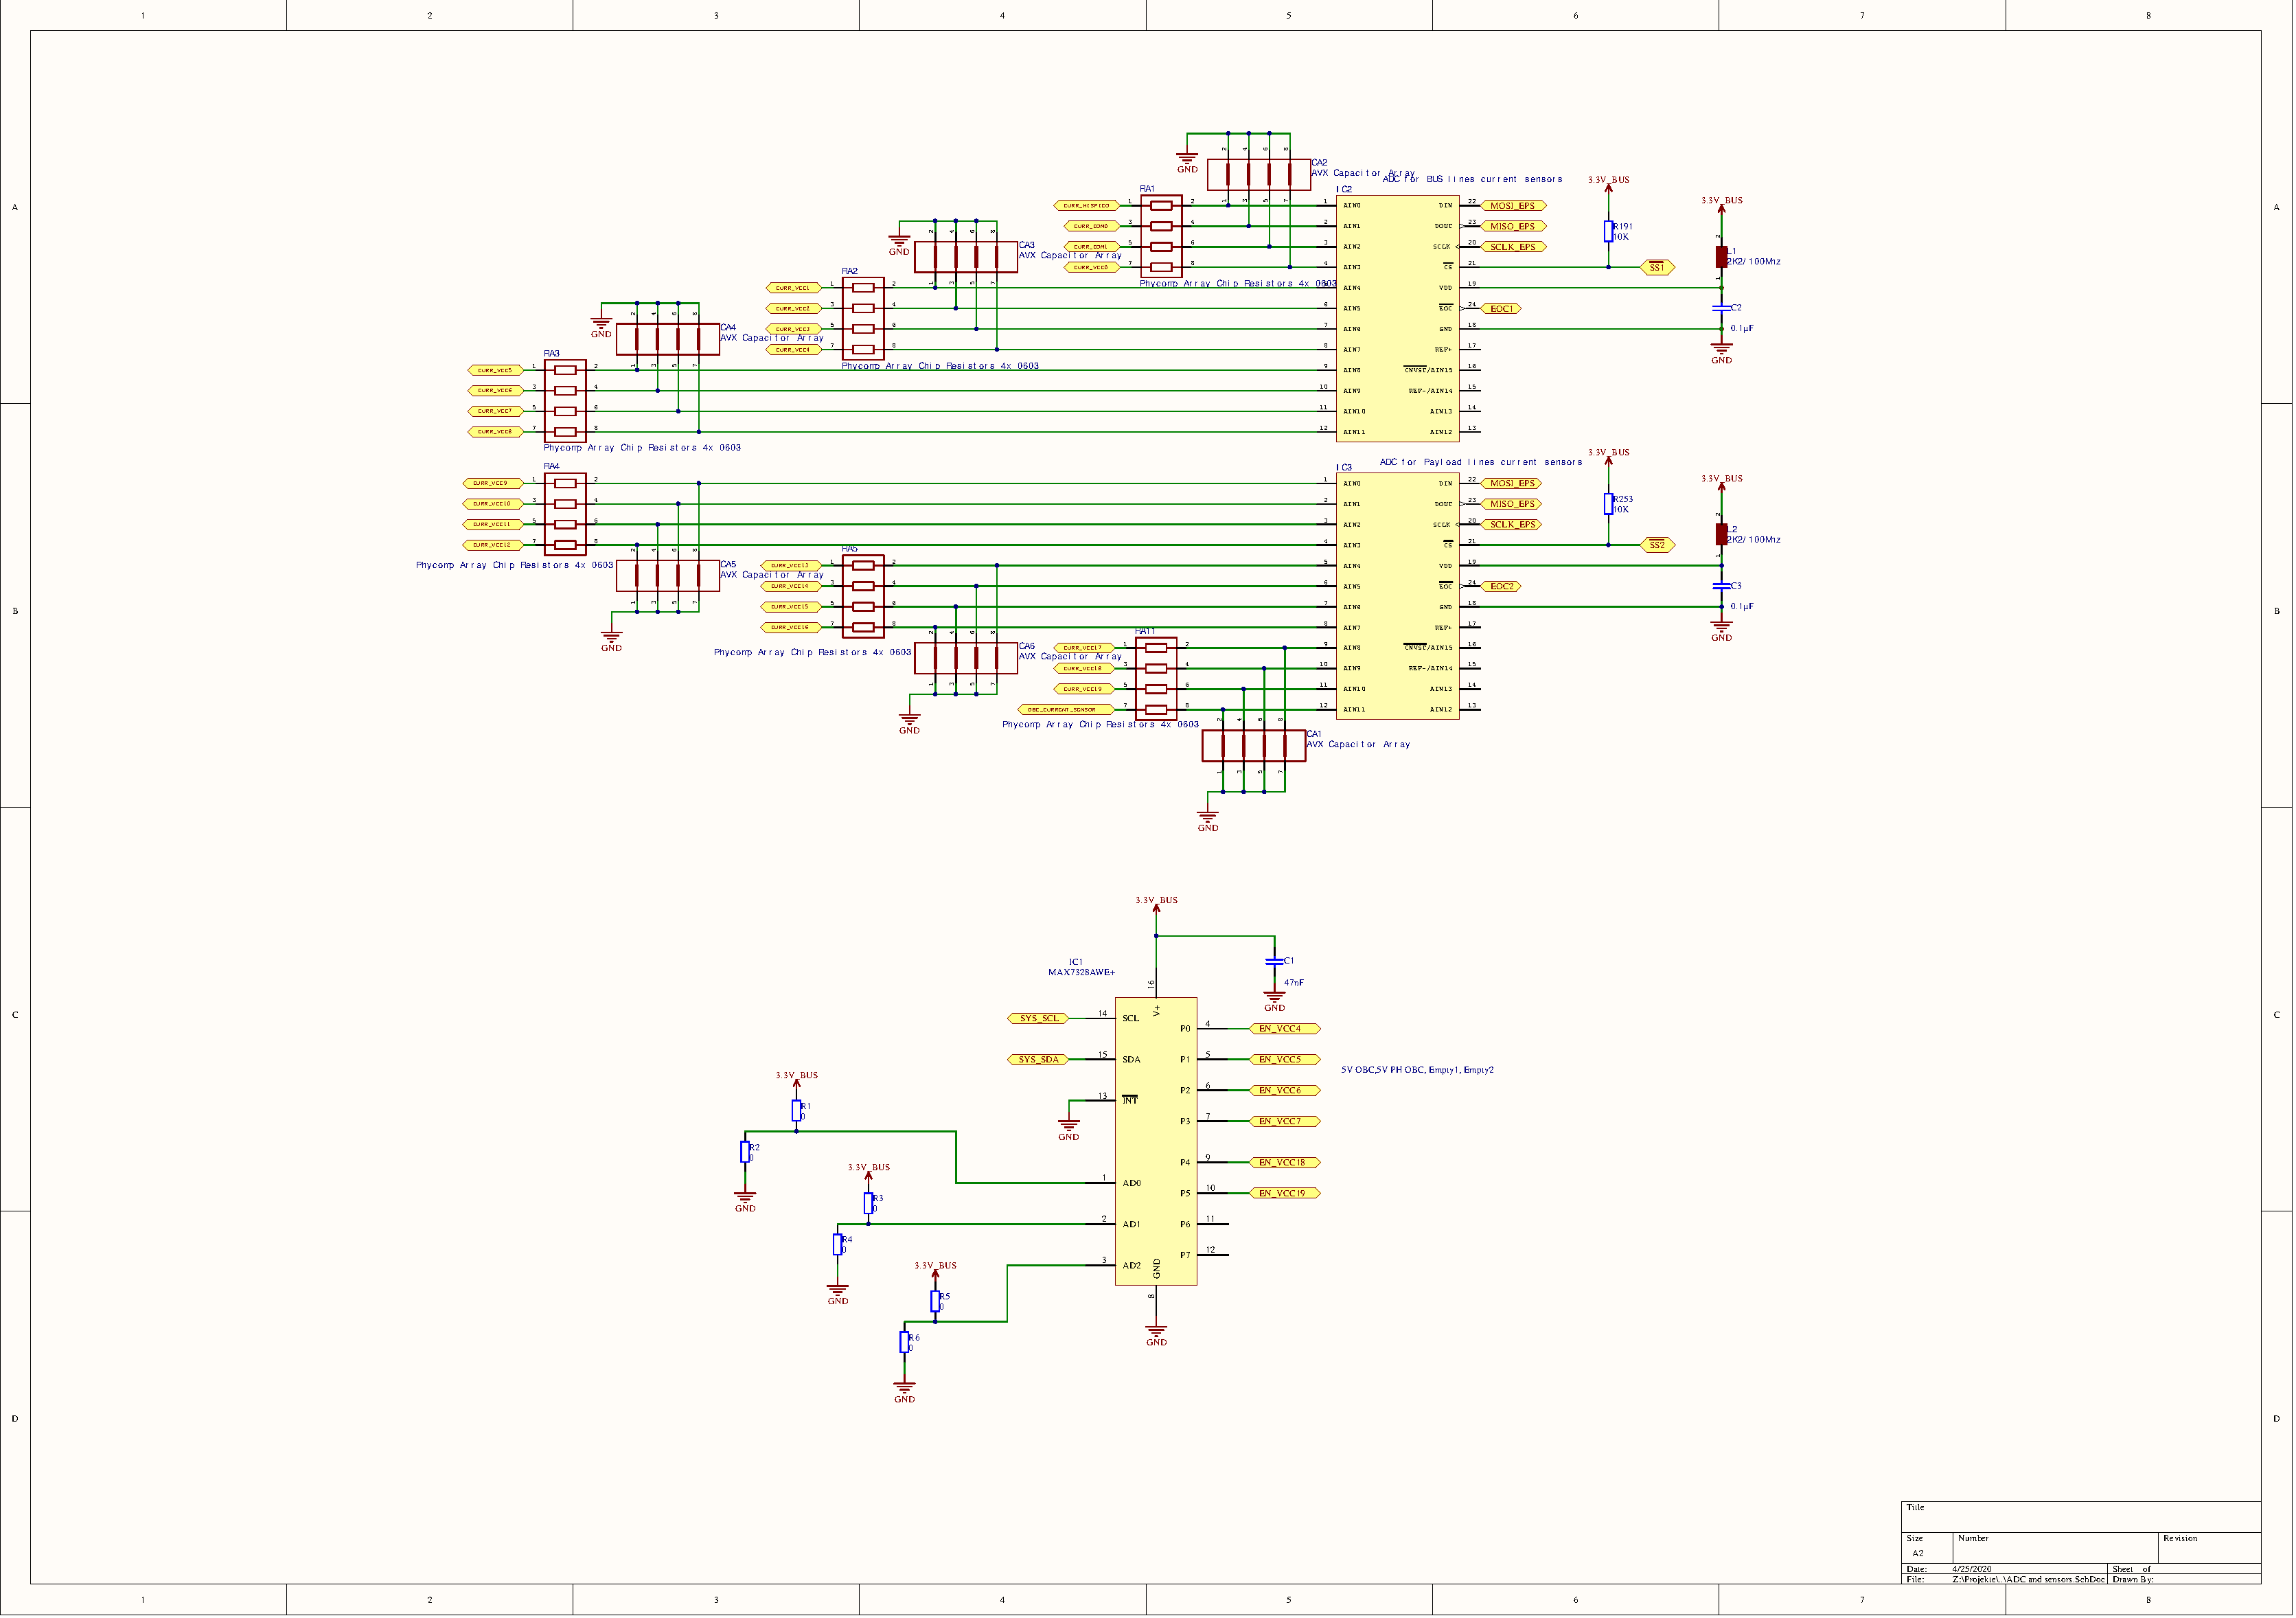
\includepdf[pages=1, scale=0.7, pagecommand={}, angle=90]{Job1.PDF}
\includepdf[pages=3, scale=0.7, pagecommand={}, angle=90]{Job1.PDF}
\includepdf[pages=4, scale=0.7, pagecommand={}, angle=90]{Job1.PDF}
\includepdf[pages=5, scale=0.7, pagecommand={}, angle=90]{Job1.PDF}
\includepdf[pages=7, scale=0.7, pagecommand={}, angle=90]{Job1.PDF}

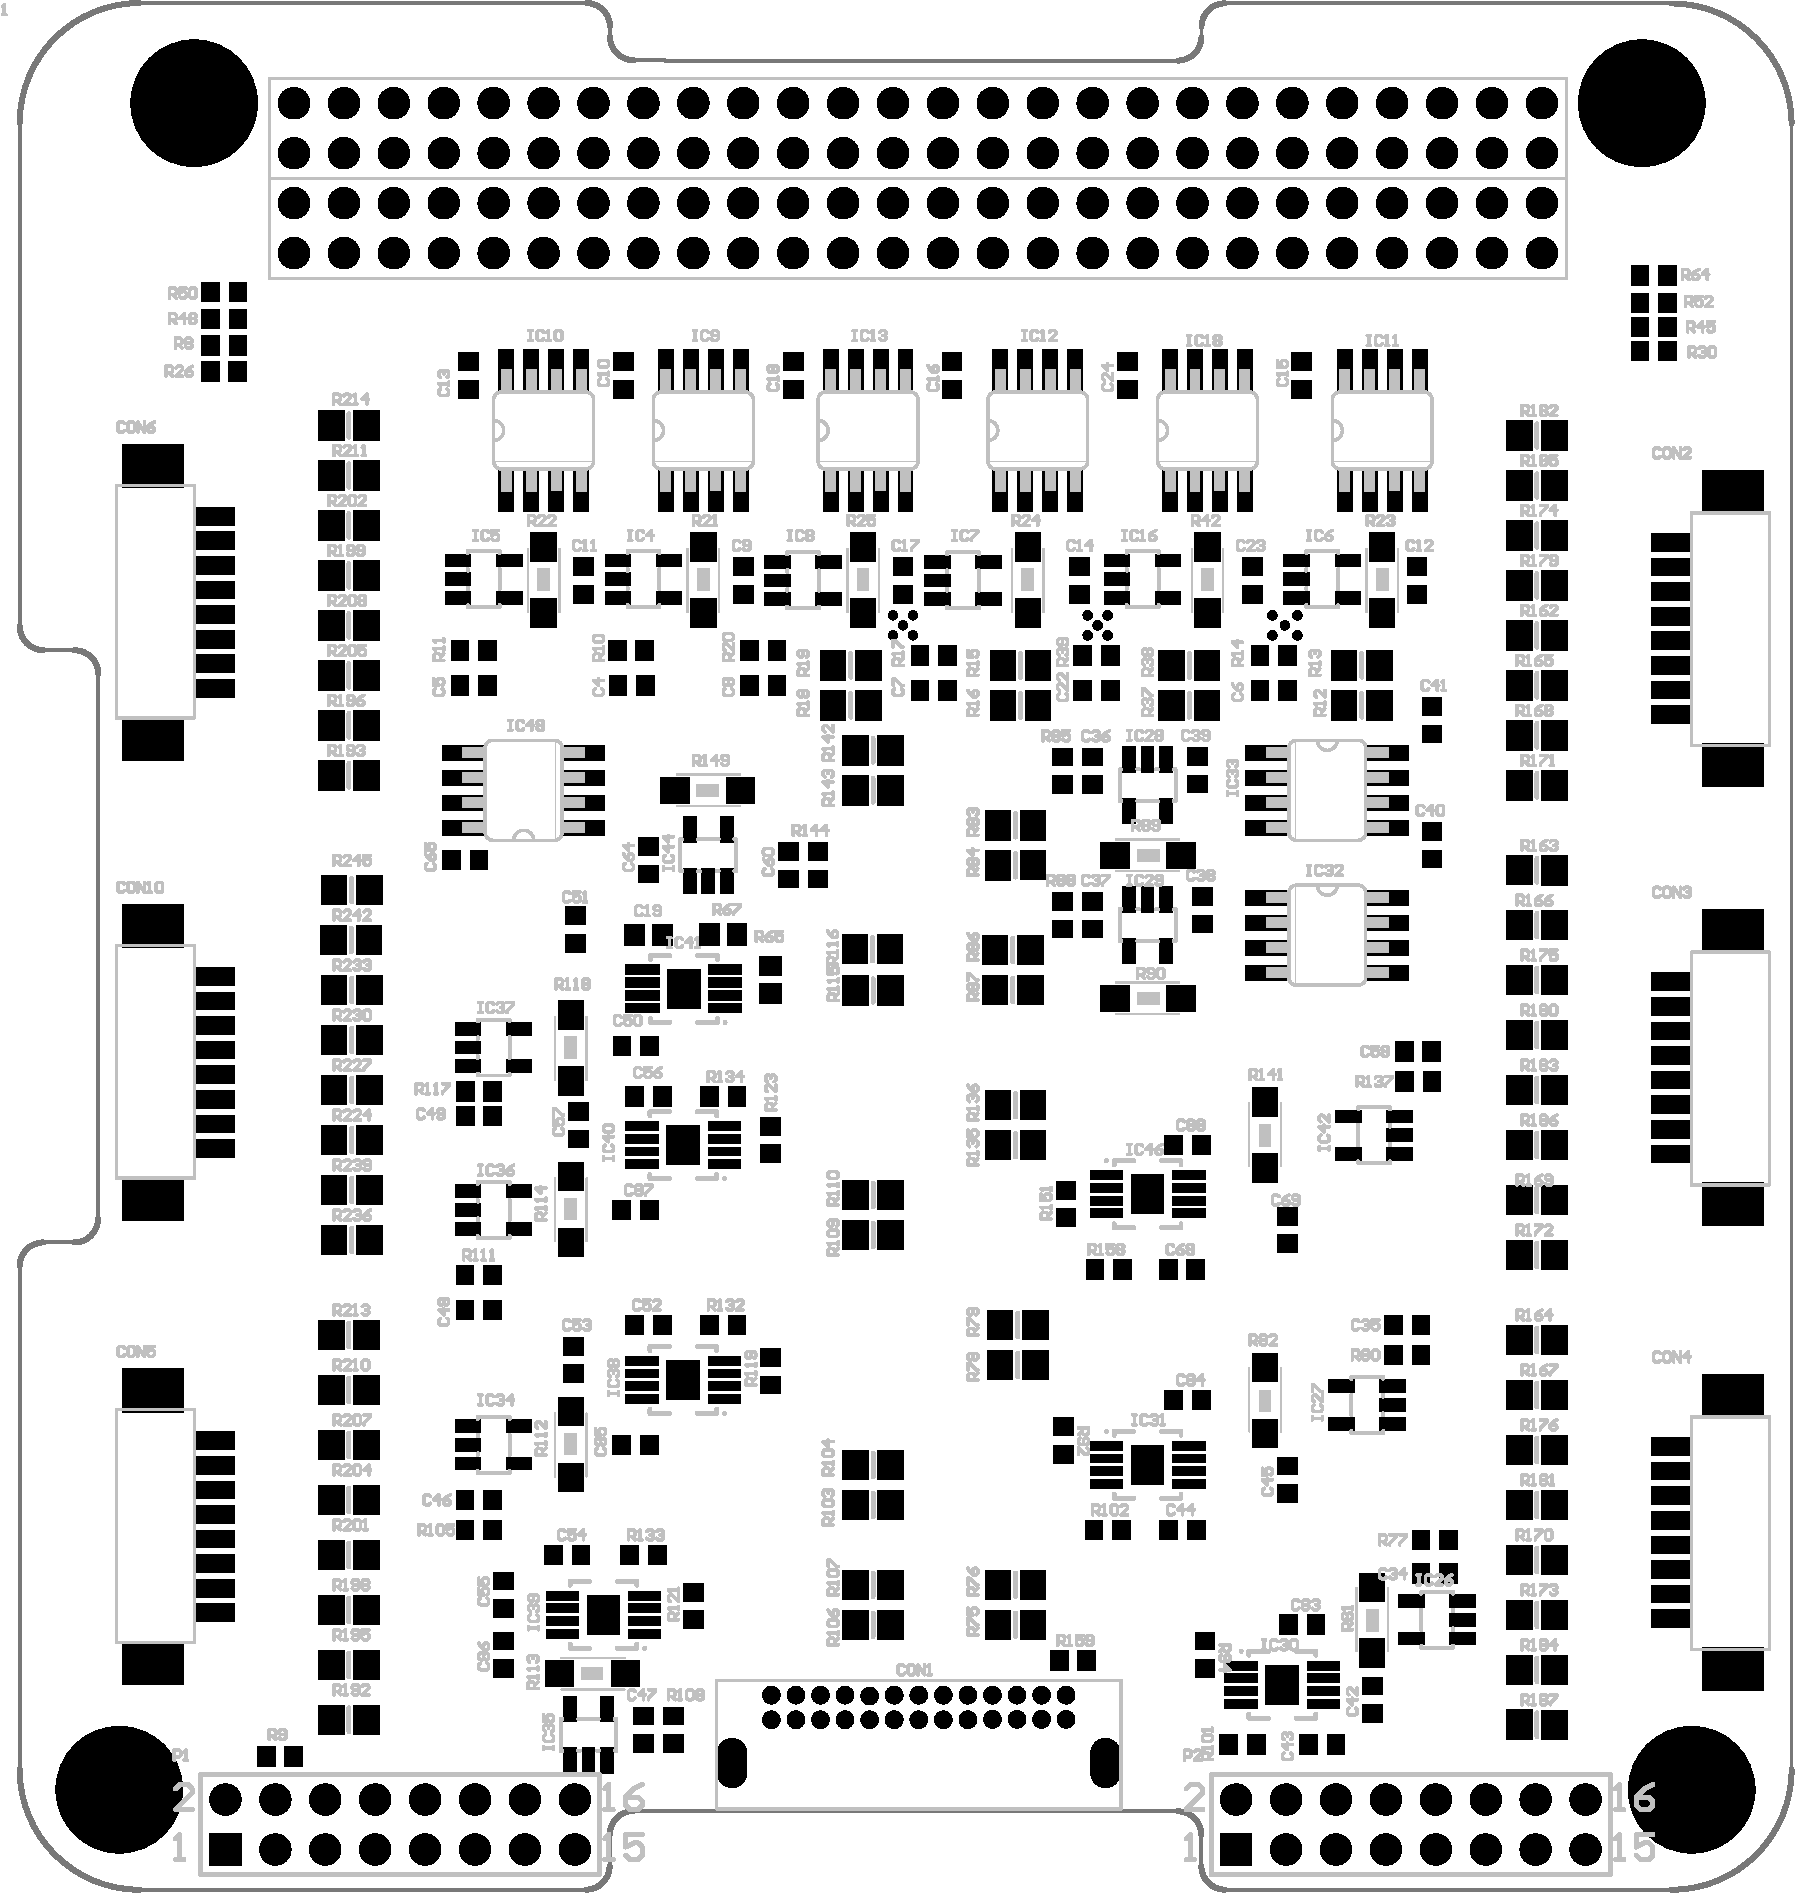
\includepdf[pages=1, scale=0.7, pagecommand={},  pagecommand=\section*{Appendix C}]{pcb2.PDF}
\includepdf[pages=2, scale=0.7, pagecommand={}]{pcb2.PDF}
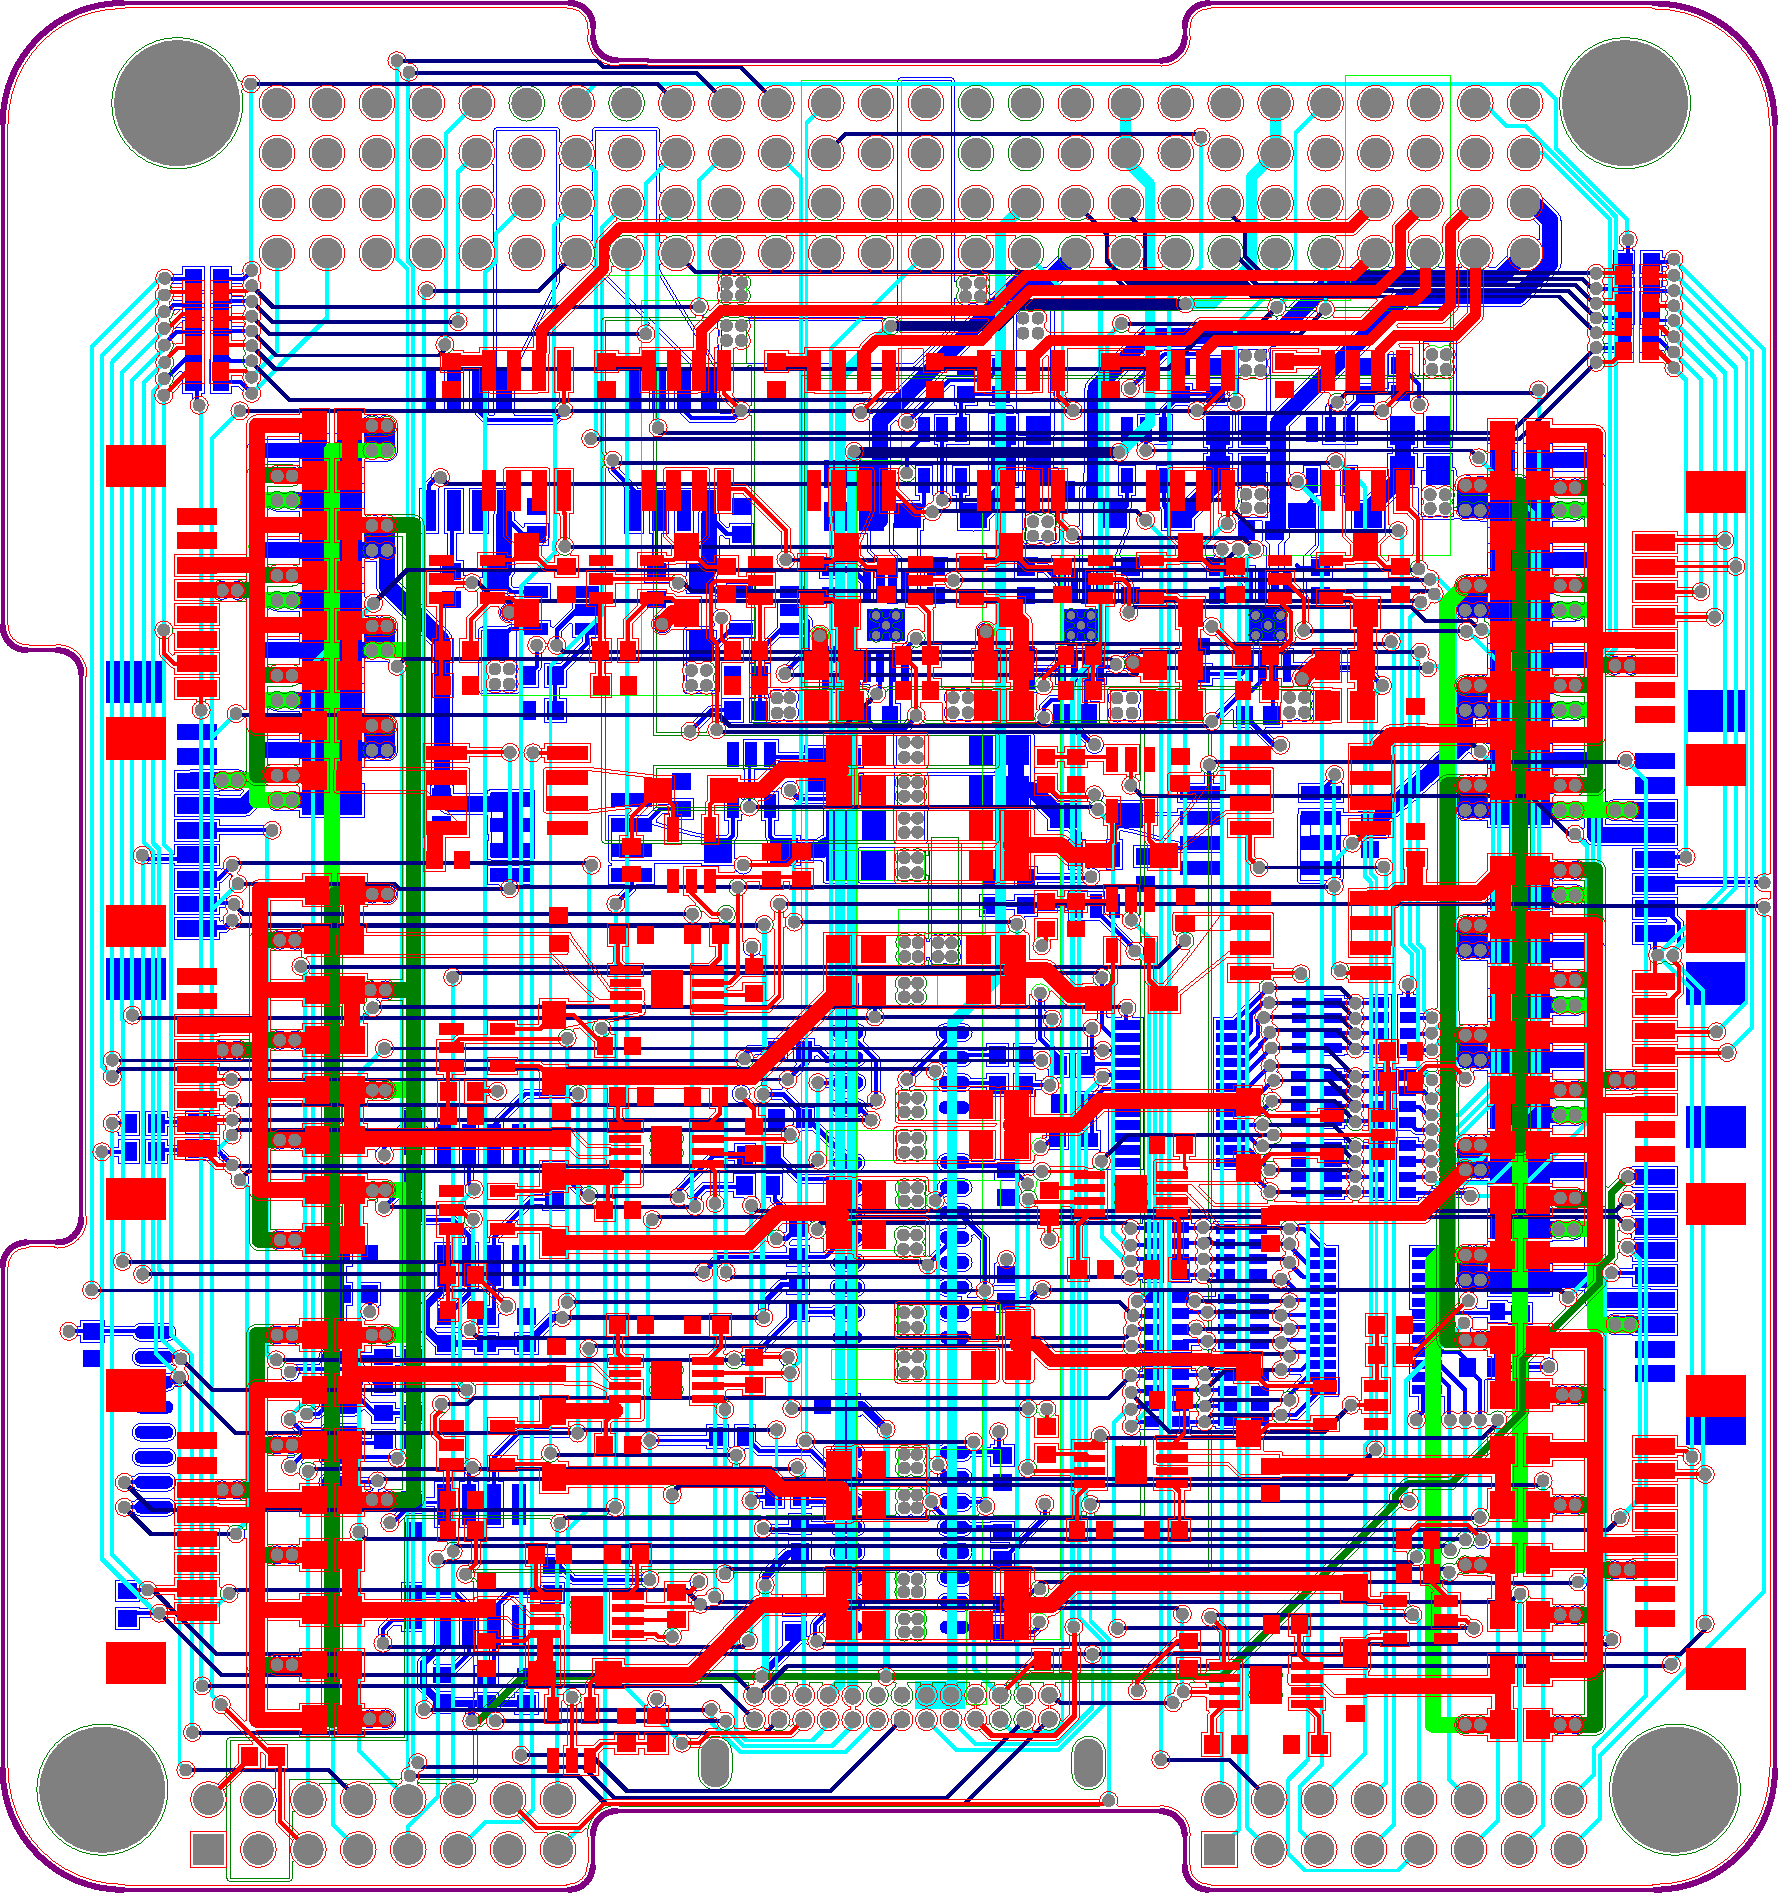
\includepdf[pages=1, scale=0.7, pagecommand={}]{pcb1.PDF}


\end{appendix}

\endinput
